\section{Principes de bases des systèmes radar et de l'imagerie SAR}
\subsection{Rappels radar}

\begin{figure}[ht]
    \centering
    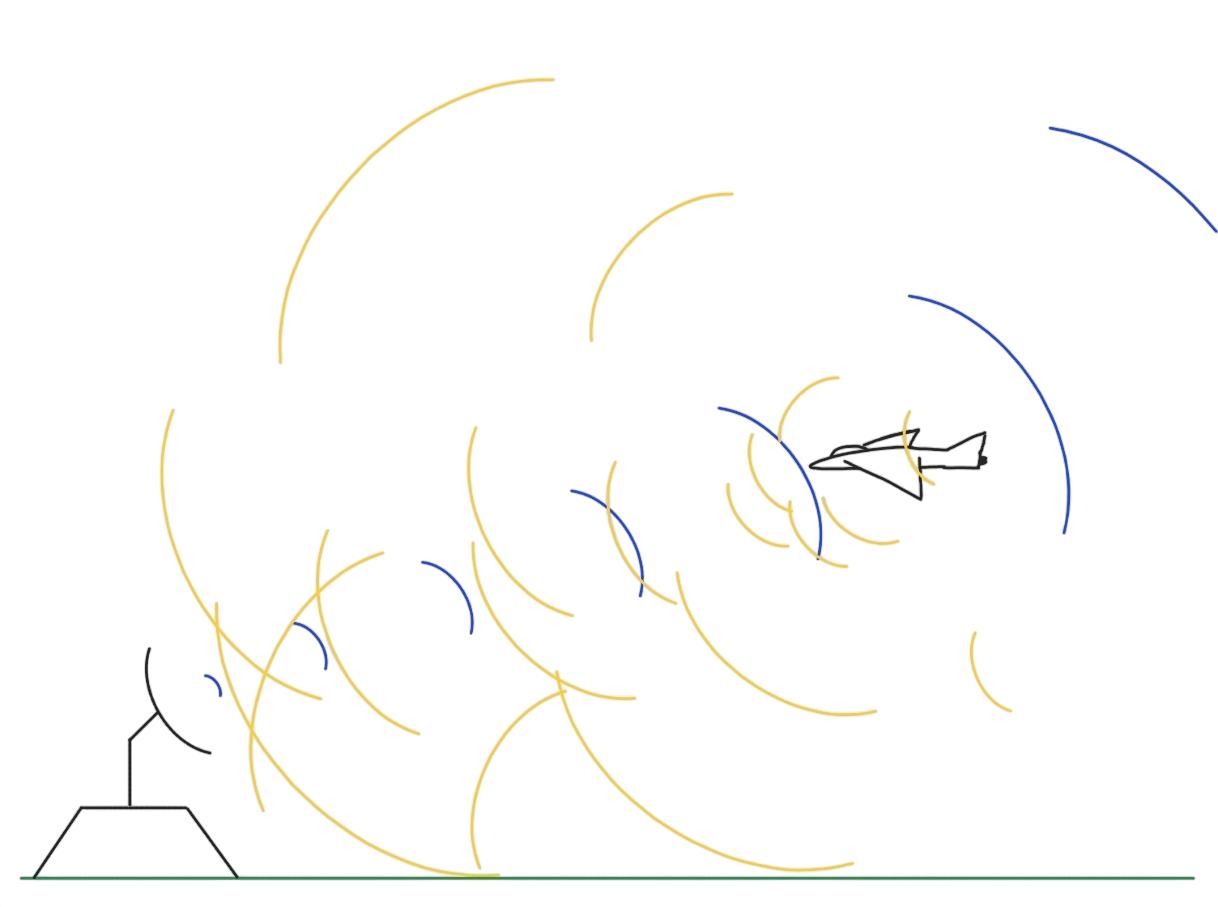
\includegraphics[width=0.5\linewidth]{src/biblio_sar/img/schema_base_radar.png}
    \caption{Schéma d'explication des bases d'un système radar}
    \label{fig:schema_explicatif_radar}
\end{figure}


Équation radar :

Pourquoi mettre "proportionnel à" alors que l'équation radar ajoute "simplement" un facteur $\frac{1}{(4\pi)^3}$ ?

\begin{equation}
    P_r \propto \frac{P_t \times G^2 \times \lambda^2 \sigma}{R^4}
\end{equation}
Où : 
\begin{description}
    \item[$P_r$] : est la puissance reçue par l'antenne [$W$]
    \item[$P_t$] : est la puissance transmise par l'antenne [$W$]
    \item[$G$] : est le gain de l'antenne (émission/réception) [$/$]
    \item[$\lambda$] : est la longueur d’onde [$m$]
    \item[$\sigma$] : est la surface équivalente radar [$m^2$]
    \item[$R^4$] : est la distance entre l'antenne et la cible [$m$]
\end{description}


Antenne :

Angle ouverture : 
\begin{equation}
    \theta \approx \frac{\lambda}{L}
\end{equation}
Où :
\begin{description}
    \item[$\theta$] : est l'angle d'ouverture [\textdegree]
    \item[$\lambda$] : est la longueur d’onde [$m$]
    \item[$L$] : est la taille physique de l'antenne [$m$]
\end{description}

Résolution range/radial :

Que veut dire le B ? Le bruit ? 

\begin{equation}
    \delta_{range} \approx \frac{c}{2B}
\end{equation}
Où :
\begin{description}
    \item[$\delta_{range}$] : est la résolution en range [$m$]
    \item[$\lambda$] : est la longueur d’onde [$m$]
    \item[$L$] : est la taille physique de l'antenne [$m$]
\end{description}

Résolution en azimut/latérale :

\begin{equation}
    \delta_{az} \approx \frac{R\times \lambda}{L}
\end{equation}
Où :
\begin{description}
    \item[$\delta_{az}$] : est la résolution azimutale [$m$]
    \item[$R$] : est la distance entre l'antenne et la cible [$m$]
    \item[$\lambda$] : est la longueur d’onde [$m$]
    \item[$L$] : est la taille physique de l'antenne [$m$]
\end{description}

Résolution Approximée car la résolution n'est pas la même partout sur la fauchée/tache au sol.

radar cw,
impulsion
chirp
doppler
fmcw
radar pulsé (impulsion ???)

\subsection{Limites des radars conventionnels pour l'imagerie}

\subsection{Principe du SAR}

Rappels radar : portée, Doppler, résolution, SNR.

Limites des radars conventionnels pour l’imagerie.
speckle (chatoiement) 

Principe du SAR : ouverture synthétique, compression en distance et en azimut.




\newpage
1. Introduction

Contexte général : radar, observation tout temps, intérêt civil et militaire.

Besoin d’imagerie haute résolution → limites des radars conventionnels → motivation du SAR.

Positionnement spécifique : SAR embarqué sur drones, multi-capteurs, fusion et détection.

2. Principes de base du radar et du SAR

Rappels radar : portée, Doppler, résolution, SNR.

Limites des radars conventionnels pour l’imagerie.
speckle (chatoiement) 

Principe du SAR : ouverture synthétique, compression en distance et en azimut.

3. Algorithmes de traitement SAR (formation d’image)
3.1 Compression en distance et en azimut
3.2 Algorithmes classiques

Range-Doppler

Chirp Scaling

omega–k (Range Migration Algorithm)

Backprojection

3.3 Limitations et hypothèses

Trajectoire rectiligne idéale, scène plane, hypothèse cible ponctuelle.

Contraintes en bande, navigation et coût calcul.

3.4 Comparaison des algorithmes
4. Avancées récentes en traitement SAR

Compensation de mouvement (MOCO), autofocus.

Traitements temps-fréquence et robustes.

Implémentations temps réel (GPU, FPGA).

Approches émergentes (IA, deep learning pour focalisation).

5. SAR embarqué sur drones (UAV-SAR)
5.1 Intérêt et spécificités

Portabilité, observation basse altitude, flexibilité.

5.2 Contraintes UAV

Masse/énergie, vibrations, trajectoire non idéale, volume de données.

5.3 Travaux académiques (ex. Pelle 2020, projets universitaires)
5.4 Développements industriels (mini-SAR sur drones militaires et civils)
5.5 Algorithmes adaptés

Backprojection robuste, navigation assistée GNSS/IMU, correction post-traitement.

6. Fusion multi-drones et SAR collaboratif
6.1 Intérêt : couverture étendue, redondance, meilleure résolution.
6.2 Contraintes : synchronisation temporelle, cohérence de phase, calibration inter-capteurs.
6.3 Travaux existants : MIMO-SAR, expériences UAV multi-capteurs.
6.4 Limites actuelles et défis pour l’avenir.
7. Détection en imagerie SAR
7.1 Objectif et enjeux de la détection

Cibles ponctuelles vs étendues, clutter, hétérogénéité du milieu.

7.2 Algorithmes classiques de détection

CFAR (CA-CFAR, OS-CFAR, GO-CFAR, SO-CFAR).

Détection par seuillage global et adaptatif.

7.3 Limites des méthodes classiques

Environnements hétérogènes, forte densité de clutter, faible SNR.

7.4 Approches avancées

Détection bayésienne et probabiliste.

Exploitation de l’information polarimétrique/interférométrique.

Apprentissage automatique (SVM, réseaux de neurones).

Deep learning pour la détection et classification d’objets dans les images SAR.

7.5 Évaluation des performances

Probabilité de détection (Pd), taux de fausses alarmes (Pfa).

Jeux de données et benchmarks (MSTAR, OpenSAR, etc.).

8. Discussion et perspectives

Comparaison des approches (formation image vs exploitation).

Verrous scientifiques actuels : navigation précise, traitement distribué, robustesse en clutter.

Perspectives : SAR multi-drones collaboratifs, IA pour fusion + détection en temps réel.

9. Conclusion

Synthèse des connaissances actuelles.

Positionnement de ton projet par rapport à l’état de l’art.